%! Author = Filippo Vissani
%! Date = 08/02/24
% !TeX root = ../thesis-main.tex

%----------------------------------------------------------------------------------------
\chapter{Background}
\label{chap:background}
%----------------------------------------------------------------------------------------

This chapter provides a broad overview of the concepts, paradigms, and frameworks that served as points of reference during the entire development of this thesis.

\section{Functional Programming}

The functional paradigm, in the context of computer science, involves building programs through the application and composition of functions. It adopts a declarative approach, where function definitions are represented as trees of expressions mapping values to other values, rather than relying on a sequence of imperative statements to update the program's running state.

\subsection{Concepts}

This section elucidates fundamental concepts that form the basis of functional programming.

\paragraph{Higher-order functions}

Higher-order functions possess the ability to either receive functions as arguments or produce them as results. The nuanced difference lies in the mathematical concept denoted by "higher-order", which involves functions operating on other functions.

These functions facilitate partial application or currying, enabling a technique where a function is applied to its arguments one at a time. With each application, a new function is created to handle the next argument. This approach allows programmers to express ideas succinctly, such as representing the successor function by partially applying the addition operator to the natural number one.

\paragraph{Purity}
Pure functions, or expressions, lack side effects. This absence of side effects endows pure functions with various advantageous properties, many of which can be leveraged for code optimization. A pure function, to be defined as such, must meet the following properties:

\begin{itemize}
    \item If the result of a pure expression is not used, it can be removed without influencing other expressions.
    \item If a pure function is invoked with arguments that do not introduce side effects, the result remains constant concerning that set of arguments. Repeatedly calling the pure function with the same arguments yields identical results.
\end{itemize}

\paragraph{Recursion}

Functional languages typically employ recursion for iteration. Recursive functions call themselves, allowing an operation to iterate until it meets the base case. Generally, recursion involves managing a stack, consuming space proportional to the recursion depth. This characteristic might render recursion less favorable compared to imperative loops due to potential space inefficiency. Nonetheless, a specific type of recursion called tail recursion can be identified and optimized by a compiler, producing code similar to that used for iteration in imperative languages. Implementing tail recursion optimization involves transforming the program using a continuous passing style during compilation.

\paragraph{Evaluation strategies}

In functional languages, various methods are commonly provided for evaluating arguments during their passage to functions. Three primary approaches include:

\begin{itemize}
    \item \textit{Call-by-value}: This involves evaluating arguments before the function application.
    \item \textit{Call-by-name}: Here, arguments are assessed each time their value is needed within the function body.
    \item \textit{Call-by-need}: Also known as lazy evaluation, this approach involves evaluating arguments only when their value is first required within the function body.
\end{itemize}

\paragraph{Type systems}

Functional programming languages have leaned towards employing typed lambda calculus. This approach involves rejecting all invalid programs at compilation time, even at the risk of encountering false positive errors. In contrast, untyped lambda calculus, accepts all valid programs at compilation time, running the risk of false negative errors, as it rejects invalid programs only at runtime when there is sufficient information to distinguish valid from invalid programs. The incorporation of algebraic data types enhances the ease of manipulating complex data structures. Additionally, the robust compile-time type checking contributes to program reliability, offering a level of assurance even in the absence of other reliability techniques. Furthermore, type inference alleviates the need for manual declaration of types by the programmer in most cases.

\paragraph{Referential transparency}

In functional programming, there are no assignment statements; once a variable is defined, its value remains constant throughout the program's execution. This characteristic eliminates the possibility of side effects since any variable can be substituted with its actual value at any given point in the program. Consequently, functional programs are characterized by referential transparency.

\paragraph{Data structures}

Purely functional data structures are often represented differently from their imperative counterparts. While arrays, providing constant access and update times, are fundamental in most imperative languages, purely functional alternatives might employ maps or random access lists. Although these alternatives allow for a purely functional implementation, they come with logarithmic access and update times. One distinguishing feature of purely functional data structures is persistence, which involves maintaining unmodified previous versions of the data structure.

\subsection{Functional Programming in Kotlin}

Kotlin, an open-source programming language characterized by static typing, accommodates both object-oriented and functional programming paradigms. Rather than striving for uniqueness, Kotlin derives inspiration from decades of language development. Variants of Kotlin are designed to target different platforms, including the \ac{jvm}, JavaScript, and native code.

In Kotlin, functions are treated as first-class entities, implying their ability to be stored in variables and data structures. Additionally, they can be passed as arguments to and returned from other higher-order functions. The operations that can be performed on functions are equivalent to those applicable to other non-function values.

To support these functionalities, Kotlin, being a statically typed programming language, employs a family of function types to represent functions. Moreover, it incorporates specialized language constructs, such as lambda expressions.

An illustrative instance of a higher-order function in Kotlin is the functional programming idiom \texttt{fold} (\Cref{lst:fold-function})
employed for collections. This function receives an initial accumulator value and a combining function. Subsequently, it constructs its return value by iteratively combining the current accumulator value with each element in the collection. Importantly, the accumulator value is replaced with each iteration.

\lstinputlisting[float,language=Kotlin,label={lst:fold-function},caption= \texttt{fold} function]{listings/fold.kt}

the \texttt{combine} parameter has the function type \((R, T) \rightarrow R\), so it accepts a function that takes two arguments of types \textit{R} and \textit{T} and returns a value of type \textit{R}. It is invoked inside the \texttt{for} loop, and the return value is then assigned to \texttt{accumulator}.

Kotlin uses function types, such as \((Int) \rightarrow String\), for declarations that deal with functions. Each function type in Kotlin is characterized by a parenthesized list specifying the parameter types and a return type. For example, \((A, B) \rightarrow C\) represents a type indicative of functions that accept two arguments of types \textit{A} and \textit{B}, yielding a result of type \textit{C}. The parameter list may be empty, denoted by \(() \rightarrow A\). It is essential to note that the return type cannot exclude the declaration of \texttt{Unit}. Function types have the option to include an additional receiver type, indicated before the dot in the notation. For instance, the type \(A.(B) \rightarrow C\) signifies functions that can be invoked on a receiver object \textit{A}, accepting a parameter \textit{B}, and producing a result of type \textit{C}.

\section{Reactive Programming}

Reactive programming, as defined in~\cite{Bainomugisha2013}, is a programming paradigm centered on the concept of continuous time-varying values and the seamless propagation of changes. It streamlines the declarative creation of event-driven applications by enabling developers to articulate programs in terms of desired actions, leaving it to the language to autonomously handle the timing of execution. Within this paradigm, alterations in the state are automatically and efficiently disseminated throughout the network of interdependent computations by the intrinsic execution model.

Consider the example of calculating the sum of two variables (\Cref{lst:reactive-example}). In conventional sequential imperative programming, the value of the variable \texttt{var3} will always contain 3, which is the sum of the initial values of variables \texttt{var1} and \texttt{var2} even when \texttt{var1} or \texttt{var2} is later assigned a new value (unless the programmer explicitly assigns a new value to the variable \texttt{var3}). In reactive programming, the value of the variable \texttt{var3} is always kept up-to-date. In other words, the value of \texttt{var3} is automatically recomputed over time whenever the value of \texttt{var1} or \texttt{var2} changes.
This is the key notion of reactive programming. Values change over time and when they change all dependent computations are automatically reexecuted. In reactive programming terminology, the variable \texttt{var3} is said to be dependent on the variables \texttt{var1} and \texttt{var2}.

\lstinputlisting[float,label={lst:reactive-example},caption=Example of a program with reactive values]{listings/reactive-example.txt}

\subsection{Evaluation Model}

The evaluation model of a reactive programming language focuses on how changes propagate across a dependency graph of values and computations. From the programmer's perspective, the automatic propagation of changes is a fundamental aspect of reactive programming. Essentially, any alteration in a value should be automatically transmitted to all computations dependent on it. When an event occurs at a source, computations reliant on that event should be notified of the changes, potentially triggering a recomputation.

At the language level, a crucial design decision involves determining who initiates the propagation of changes. This entails deciding whether the source should \textit{push} new data to its dependents (consumers) or if the dependents should \textit{pull} data from the event source (producer). In the pull-based model, the computation that requires a value needs to ``pull" it from the source. That is, propagation is driven by the demand for new data. In the push-based model, when the source has new data, it pushes the data to its dependent computations. That is, propagation is driven by the availability of new data.

\subsection{Reactive Operators}

The primary advantage offered by libraries furnishing the reactive streams APIs lies in the provision of operators. These operators are essentially functions applicable to a data stream, adept at solving problems related to the processing of reactive streams, encompassing tasks such as filtering, mapping (\Cref{fig:reactive-map}), and aggregating.

Furthermore, these operator functions are intentionally designed to be composable, signifying their capability to be consecutively linked to construct processing pipelines. Each operator function receives an observable as input and yields another observable as output. Consequently, the outcome of one operator function can seamlessly serve as the input for another operator function, a concept termed operator chaining.

\begin{figure}
    \centering
    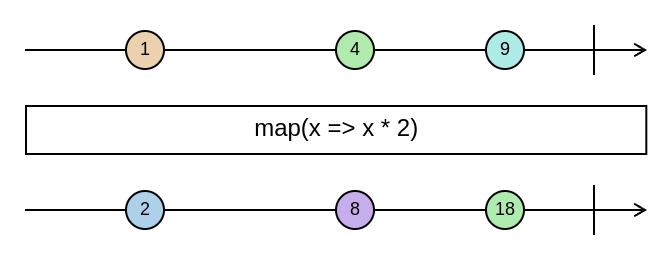
\includegraphics[width=\linewidth]{figures/map-marble.png}
    \caption{Map operator in reactive applications}
    \label{fig:reactive-map}
\end{figure}

\subsection{Reactive Programming in Kotlin}

Kotlin\footnote{\url{https://kotlinlang.org/}} Flow\footnote{\url{https://kotlinlang.org/docs/flow.html}} is a part of the Kotlin Coroutines library, introduced to provide a reactive programming model for asynchronous \textit{cold}\footnote{A flow that emits values only when there is an active collector.} and \textit{hot}\footnote{A flow that produces values regardless of whether there are active collectors.} data streams.

A \texttt{Flow} is an asynchronous data stream that sequentially emits values and completes normally or with an exception. Intermediate operators on the flow such as \texttt{map}, \texttt{filter}, \texttt{take} and \texttt{zip} are functions that are applied to the \textit{upstream} flow or flows and return a \textit{downstream} flow where further operators can be applied to. Intermediate operations do not execute any code in the flow and are not suspending functions\footnote{A function that can be paused and resumed at a later time.} themselves. They only set up a chain of operations for future execution and quickly return. This is known as a cold flow property. \textit{Terminal operators} on the flow are either suspending functions such as \texttt{collect}, \texttt{single}, \texttt{reduce} and \texttt{toList} or \texttt{launchIn} operator that starts collection of the flow in the given scope. They are applied to the upstream flow and trigger the execution of all operations. Execution of the flow is also called ``collecting the flow" and is always performed in a suspending manner without actual blocking. Terminal operators complete normally or exceptionally depending on the successful or failed execution of all the flow operations in the upstream.

By default, flows are \textit{sequential} and all flow operations are executed sequentially in the same coroutine\footnote{A concurrency design pattern that allows to write asynchronous, non-blocking code in a sequential style.}, with an exception for a few operations specifically designed to introduce concurrency into flow execution such as \texttt{buffer} and \texttt{flatMapMerge}.

The \texttt{Flow} interface does not carry information on whether a flow is a cold stream that can be collected repeatedly and triggers execution of the same code every time it is collected, or if it is a hot stream that emits different values from the same running source on each collection. Usually flows represent cold streams, but there is a \texttt{SharedFlow} subtype that represents hot streams. In addition to that, any flow can be turned into a hot one by the \texttt{stateIn} and \texttt{shareIn} operators, or by converting the flow into a hot channel via the \texttt{produceIn} operator.

The example \Cref{lst:flow-example} demonstrates the asynchronous nature of Kotlin Flow and how it allows concurrent execution without blocking the main thread. The \texttt{simple} function creates a flow using the \texttt{flow} builder. Inside the flow, it emits values from 1 to 3 with a delay of one hundred milliseconds between each emission. The delay simulates an operation that takes time, such as network calls or disk I/O. In the \texttt{main} function, a coroutine is launched using \texttt{launch} to run concurrently with the main thread. This coroutine prints messages indicating that it's not blocked and introduces delays between each message. As the flow is collected in the main coroutine, the emitted values are printed and interleaved with the messages from the concurrent coroutine (\Cref{lst:flow-example-result}). This demonstrates that the main thread is not blocked during the execution of the flow, thanks to the asynchronous nature of flows.

\lstinputlisting[float,language=Kotlin,label={lst:flow-example},caption=Kotlin Flow example]{listings/flow-example.kt}

\lstinputlisting[float,label={lst:flow-example-result},caption=Kotlin Flow example result]{listings/flow-example-result.txt}

\section{Aggregate Computing}

\textit{Aggregate computing} is a method for designing intricate coordinations in distributed systems, particularly for \textit{\ac{cas}}. The approach primarily centers on the notion that understanding system interactions is more straightforward when viewed in the context of information flowing through groups of devices, as opposed to focusing on individual devices and their interactions with peers and the environment.~\cite{Viroli2019}

Aggregate computing is especially suitable for scenarios where the problem at hand involves a network of devices possessing the following characteristics:

\begin{itemize}
    \item \textbf{Openness}, indicating that the surrounding environment where devices operate can undergo unforeseen changes and faults.
    \item \textbf{Large scale}, involving a potentially extensive number of devices or agents that necessitate effective abstractions for coordination.
    \item \textbf{Intrinsic adaptiveness}, signifying the capability to respond to significant events to ensure the overall resilience of the system.
\end{itemize}

Addressing these considerations requires an approach grounded in \textit{self-organization}, where cohesive and resilient coordination behavior arises from localized coordination abstractions. Another objective of aggregate computing is to provide developers with a means to articulate the behavior of distributed systems possessing the aforementioned features in a composable and declarative manner. This facilitates better scalability in dealing with the intricacies of the domain. The mathematical foundation of aggregate computing, relying on \textit{\ac{fc}} (\Cref{subsection:field-calculus}), enables this capability.

\subsection{Abstractions}
\label{subsection:abstractions}

Aggregate computing models a distributed system as a set $\mathcal{D}$ of devices, ranged over by $\delta$. On top of that, a reflexive~\footnote{each device is a neighbor of itself.} \textit{neighboring relation} indicates the devices with which one can communicate (which is application-dependent and can be used to describe logical or physical proximity). In addition, each device has a set of \textit{sensors} that enable the perception of the environment.

The primary abstraction introduced by aggregate computing is the \textit{computational field} (or simply \textit{field}), which is a function $\phi: \mathcal{D} \mapsto \mathcal{L}$ mapping each device $\delta \in \mathcal{D}$ to a local value $l \in \mathcal{L}$~\cite{Viroli2018}.
%
A \textit{field evolution} is a dynamically changing field, and a \textit{field computation} takes field evolutions as inputs and produces field evolutions as outputs.
%
These outputs are defined in such a way that they change tracking input changes.

The key idea of aggregate computing is that any field computation (\textit{global interpretation}) can be mapped to a \textit{single-device behavior} that is iteratively executed by all the devices in the network (\textit{local interpretation}).
%
Each iteration executed by a device is called a \textit{computation round} and can be subdivided into three steps:
%
\begin{itemize}
    \item \textbf{sense}: the device gathers information coming from its neighbors and local sensors, which are collected to create its \textit{local context} (or \textit{local state}) for the current round;
    \item \textbf{eval}: the computation defined by the behavior is evaluated against the local context, producing an \textit{export};
    \item \textbf{broadcast}: the export is broadcasted to all the device's neighbors, which in turn collect and use this information in their future rounds.
\end{itemize}

\subsection{Field Calculus}
\label{subsection:field-calculus}

Aggregate computing builds from a foundation of the field calculus, a functional programming model for the specification and composition of collective behaviors with formally equivalent local and aggregate semantics.

The concept of field calculus was introduced in~\cite{Viroli2013} as a fundamental core calculus designed to encapsulate the essential elements found in languages utilizing computational fields. These include functions operating over fields, functional composition involving fields, the progression of fields over time, the creation of fields of values based on neighboring elements, and the limitation of a field computation to a specific sub-region within the network. While its syntax, typing, and semantics are deeply discussed in~\cite{Viroli2019} and are omitted here for simplicity, a brief description of its elements is presented below:

\begin{itemize}
    \item a \textit{field calculus program} $\texttt{P}$ consists of a sequence of \textit{function declarations} $\bar{\texttt{F}}$ followed by the \textit{main expression} $\texttt{e}$;
    \item an expression $\texttt{e}$ can be:
    \begin{itemize}
        \item a \textit{variable} $\texttt{x}$, e.g., a function parameter;
        \item a \textit{local value} $l$, such as a Boolean, number, string, pair, tuple, etc;
        \item a \textit{neighboring field value} $\phi$, e.g., a map of
        neighbors to the distances to those neighbors;
        \item a \textit{function call} $\texttt{f}(\bar{\texttt{e}})$ to a \textit{user-declared function} or a \textit{built-in function}, such
        as a mathematical or logical operator, a data structure operation, or a function returning the value of a sensor;
        \item a \textit{branching expression} $\texttt{if} (\texttt{e}_1)\{\texttt{e}_2\}\{\texttt{e}_3\}$ which splits computation into isolated sub-regions, resulting in $\texttt{e}_2$ where and when $\texttt{e}_1$ evaluates to true, and in $\texttt{e}_3$ otherwise;
        \item a $\texttt{nbr}(\texttt{e})$ construct, which creates a neighboring field value that maps each neighbor to the latest result of evaluating $\texttt{e}$;
        \item a $\texttt{rep}(\texttt{e}_1)\{(\texttt{x})\Rightarrow \texttt{e}_2\}$ construct, which models state evolution over time.
    \end{itemize}
\end{itemize}

To work properly, the semantics of \texttt{nbr} and \texttt{rep} require a way to access, respectively, the last registered state of each neighbor and the last registered output of the device itself. In addition, this process should be made in such a way that different instances of \texttt{rep} and \texttt{nbr} cannot inadvertently ``swap" their respective value. This process is called \textit{alignment}, and it has the consequence that two branches of an \texttt{if} expression execute in isolation, meaning that two devices that execute different branches cannot communicate with each other inside their branches. In practice, this process is done by carefully constructing the export of an expression as an \textit{evaluation tree} that represents the aggregate computation. The complete semantics of export construction and alignment can be found in Appendix C of~\cite{Viroli2018}.

\subsection{Reactive and Proactive Models}
\label{subsection:reactive-and-proactive-models}

Aggregate computing emerged as a prominent approach for programming self-organization, with the benefits of formality, abstraction, compositionality, and pragmatism. Formality stems from building the approach over field calculus with well-defined language semantics. Abstraction comes from the declarativity of the functional programming model, promoting different scheduling strategies and deployments, possibly applied automatically to different sub-activities concurrently running. Compositionality comes from adopting the functional paradigm and the field abstraction. Finally, pragmatism is supported by the language design and its separation of concerns, which enables modular DSLs and toolkits.

Though conceptually simple, the round-based model could be more efficient, because it fully re-evaluates the context and the whole program without tracking change. Though it might be acceptable for predictable patterns of environmental change, this becomes largely suboptimal for highly variable dynamics. Indeed, the round-based approach seems to be a legacy of imperative languages or solutions featuring limited compositionality. Given this motivation, taking inspiration from the functional reactive paradigm, in~\cite{Casadei2023} proposed a \textit{reactive self-organization programming language}, called FRASP (Functional Reactive Approach to Self-organization Programming), that enables the decoupling of program logic from its scheduling. The details of this programming model will be discussed more deeply in \Cref{chap:analysis}.